\chapter{Generalization of chaotic dynamics}
We begin by defining a general symbol space.
\begin{definition}
	Denote by $\Sigma^{N}$ the symbol space defined as the space of doubly infinite sequences of $N$ symbols (for $N \in \mathbb{N}$), i.e.
\begin{align}
	\boxed{
		\Sigma^{N} = \left\{ s=\ldots s_{-2} s_{-1} \bm{.} s_0s_1s_2 \ldots:\ s_i \in \{0, 1, \ldots, N-1\} \right\}.
	}
\end{align}
\end{definition}

We may constrain this symbol space by constraining which sequences are admissible. This can be done by using a transition matrix $A \in \mathbb{R}^{N \times N}$ with entries $A_{ij}\in \{0,1\}$. Then the constrained symbol space is given by
\begin{align}
	\Sigma_{A}^{N} = \left\{ s \in \Sigma^{N}:\ A_{s_i s_{i+1}} \neq 0,\forall i \right\}.
\end{align}
In the constrained space, consecutive symbols $s_i$ and $s_{i+1}$ must correspond to a 1 in the transition matrix $A$. In other words if the symbol $s_i=k$ then the symbol $s_{i+1}$ must be equal to $j$ such that $A_{kj}=1$.

\begin{ex}[Constrained symbol space]
	To demonstrate how a transition matrix can constrain the symbol space, lets start by examining $\Sigma_{A}^{2}$ for
	\begin{align}
		A =
		\begin{pmatrix}
			1 & 0 \\
			0 & 1
		\end{pmatrix}
		.
	\end{align}
	Be examining the entries of the transition matrix $A$ we find which strings are admissible
	\begin{align}
		A_{11}=1 \implies& \ldots 00\ldots \quad \textrm{admissible} \\
		A_{12}=0 \implies& \ldots 01\ldots \quad \textrm{inadmissible} \\
		A_{21}=0 \implies& \ldots 10\ldots \quad \textrm{inadmissible} \\
		A_{22}=1 \implies& \ldots 00\ldots \quad \textrm{admissible}. 
	\end{align}	
	Therefore the set $\Sigma_{A}^{2}$ is comprised only of two elements $\{\overline{0}\bm{.} \overline{0}, \overline{1}\bm{.} \overline{1}\}$. As this space is very simple and only contains fixed points of $\sigma$, no chaos can occur.
\end{ex}

\begin{definition}
	The map
	\begin{align}
		\sigma:\Sigma_{A}^{N}\to \Sigma_{A}^{N};\quad \ldots s_{-1}\bm{.} s_0 \ldots \mapsto \ldots s_{-1} s_0 \bm{.} s_1 s_2 \ldots,
	\end{align}
	is called a \emph{Bernoulli subshift of finite type} (i.e. $N< \infty $) with transition matrix $A$.
\end{definition}
Before more examination of chaos on such constrained spaces, we need to recall a definition from linear algebra.
\begin{definition}
	A matrix $A$ is called \emph{irreducible} if there exists a $k \in \mathbb{N}$ such that $\left(A^{k}\right)_{ij}\neq 0$ for every $i,j\in \{1,\ldots,N\}$.
\end{definition}

\begin{theorem}[]
	Assume that $A$ is irreducible, then 
	\begin{enumerate}
		\item $\Sigma_{A}^{N}$ is a Cantor set; and
		\item $\sigma:\Sigma_{A}^{N}\to \Sigma_{A}^{N}$ is a chaotic map.
	\end{enumerate}
\end{theorem}

Note that in the previous example with $A=I_{2}$, the transition is not irreducible, which is why chaos is not garunteed.

The role of irreducibility is critical for the theorem to work. Say for instance that the required $k$ such that each entry of $A^{k}$ is nonzero is $k=3$. Then we know that $\left(A^{3}\right)_{ij} = \sum_{l,m=1}^{3} a_{il}a_{lm}a_{mj} \neq 0$ for any pair $i,j$. Therefore there exist $l,m$ such that $a_{il}$, $a_{lm}$, and $a_{mj}$ are not equal to 0. Therefore there exists an admissible ultimate transition from state $i$ to state $j$ for all pairs $i,j$, if the symbol sequence is viewed as an itinerary. Furthermore, different irreducible transition matrices generate different types of chaos. 

\begin{ex}[Chaos in the Newton-Raphson iteration]
	Newton-Raphson iteration is a process to find the roots (zeros) of a nonlinear function $f$. The iteration is as follows
	\begin{enumerate}
		\item Start with the seed point $x_0$;
		\item Define $x_1 = x_0 - \frac{f(x_0)}{f'(x_0)}= N(x_0)$;
		\item Repeat (ii) until $x_{n+1} = N(x_{n})$.
	\end{enumerate}
	In practice this approach is often truncated when $x_{n+1}\approx N(x_{n})$. The roots of $f$ coincide with the fixed points of the 1-dimensional dynamical system $x \mapsto N(x)$. If such a fixed point ($x^{*})$ is stable \underline{and} $x_0 $ is in its domain of attraction, then $\lim_{i\to \infty }N^{i}(x_0)= x^{*}$. The iteration process is sketched in Fig. \ref{fig:NR_iteration}.
\begin{figure}[h!]
	\centering
	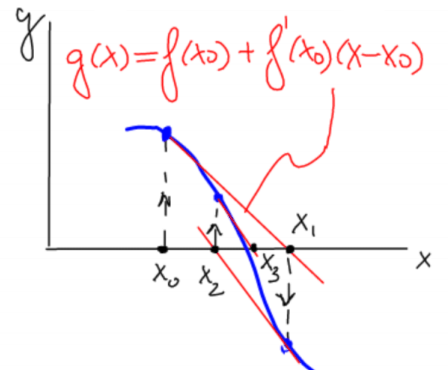
\includegraphics[width=0.4\textwidth]{figures/ch7/1NR_iteration.png}
	\caption{An illustration of the iteration of the Newton-Raphson process on the function $f$ (blue). The red designates the function $g$, when given the point $x_0$ the next iterate $x_1$ fufills the property $g(x_1)=0$.}
	\label{fig:NR_iteration}
\end{figure}

Note that if $N(x^{*}) = x^{*}$ then we have
\begin{align}
	N'(x^{*}) = 1 - \frac{f'(x^{*})^{2} - f(x^{*})f''(x_0)}{f'(x^{*})^{2}}=0.
\end{align}
The latter equality is due to $f(x^{*}) = 0$. This implies that $|N'(x^{*})|<1$, i.e. the fixed point is stable, and additional $N'(x^{*})=0$, i.e. $x^{*}$ is in fact super stable.

Specifically, once we are near the optimum $x^{*}$, we have
\begin{align}
N(x_n) = \underbrace{N(x^{*})}_{=x^{*}} + \underbrace{N'(x^{*})}_{=0}(x_n - x^{*}) + \frac{1}{2} N''(x^{*})(x_n - x^{*})^{2} + \mathcal{O}\left( | x_n - x^{*}|^{3}\right).
\end{align}
This implies we have fast quadratic convergence, as
\begin{align}
	\left| N(x_n) - N(x^{*}) \right| \approx \frac{1}{2} | N''(x^{*})| |x_{n} - x^{*}|.
\end{align}
Despite the fast convergence, erratic iterations may result if the initial point is not close enough to the root \cite{SaariUrenko}. In particular, consider a 4th order polynomial 
\begin{align}
	f(x) = (x-x_0)(x-x_1)(x-x_2)(x-x_3);\quad x_0<x_1<x_2<x_3.
\end{align}
This can be oberserved to lead to chaotic Newton-Raphson iterations.
\end{ex}

